%\documentclass[12pt]{article}

\questionheader{ex:s1.4}


%%%%%%%%%%%%%%%%%%
\subsection*{\Conceptual}
%%%%%%%%%%%%%%%%%%

%%%%%%%%%%%%%%%%%%%%%%%%%%%%%%%%
\begin{question}
The vector $\hk$ is a normal vector (i.e. is perpendicular) to the plane $z=0$. 
Find another nonzero vector that is normal to $z=0$.
\end{question}

\begin{hint}
You are looking for a vector that is perpendicular to $z=0$ and hence is
parallel to $\hk$. 
\end{hint}

\begin{answer}
Any vector of the form $c\,\hk$ with $c\ne 0$ and $c\ne 1$ works.
Three possible choices are $-\hk$, $2\,\hk$, $7.12345\,\hk$.
\end{answer}

\begin{solution}
We are looking for a vector that is perpendicular to $z=0$ and hence is
parallel to $\hk$. To be parallel of $\hk$, the vector has to be of the form $c\,\hk$ for some real number $c$.  For the vector to be nonzero, we need $c\ne 0$ and for the vector to be different from $\hk$, we need $c\ne 1$. So
three possible choices are $-\hk$, $2\,\hk$, $7.12345\,\hk$.
\end{solution}


%%%%%%%%%%%%%%%%%%%%%%%%%%%%%%%%
\begin{question}
Consider the plane $P$ with equation $3x+\frac{1}{2}y+z=4$.
\begin{enumerate}[(a)]
\item
Find the intersection of $P$ with the $y$-axis.
\item
Find the intersection of $P$ with the $z$-axis.
\item
Sketch the part of the intersection of $P$ with the $yz$-plane that is
in the first octant. (That is, with $x,y,z\ge 0$.)
\end{enumerate}
\end{question}

\begin{hint}
A point $(x,y,z)$ is on the $y$-axis if and only if $x=z=0$. Similarly,
a point $(x,y,z)$ is on the $z$-axis if and only if $x=y=0$.
\end{hint}

\begin{answer}
(a) $(0,8,0)$ \qquad
(b) $(0,0,4)$

(c)
\begin{center}
     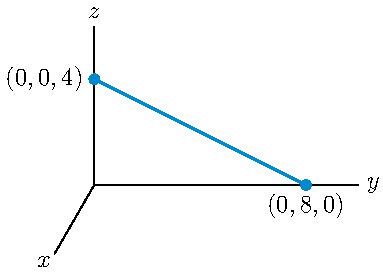
\includegraphics{intersectSketch.pdf}
\end{center}

\end{answer}

\begin{solution}
\begin{enumerate}[(a)]
\item
Each point on the $y$-axis is of the form $(0,y,0)$. Such a point is on the plane $P$ if
\begin{equation*}
3(0)+\frac{1}{2}y+0=4
\iff y=8
\end{equation*}
So the intersection of $P$ with the $y$-axis is the single point $(0,8,0)$.
\item
Each point on the $z$-axis is of the form $(0,0,z)$. Such a point is on the plane $P$ if
\begin{equation*}
3(0)+\frac{1}{2}(0)+z=4
\iff z=4
\end{equation*}
So the intersection of $P$ with the $z$-axis is the single point $(0,0,4)$.
\item
The intersection of the plane $P$ with the $yz$-plane is a line. 
We have shown in parts (a) and (b) that the points $(0,8,0)$ and $(0,0,4)$
are on that line. Here is a sketch of the part of that line that is in the first
octant.

\begin{center}
     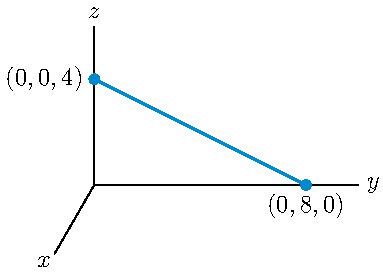
\includegraphics{intersectSketch.pdf}
\end{center}
\end{enumerate}
\end{solution}

%%%%%%%%%%%%%%%%%%%%%%%%%%%%%%%%%%%%
\begin{question}
\begin{enumerate}[(a)]
\item
Find the equation of the plane that passes through the origin and has normal vector $\llt 1,2,3\rgt$.
\item
Find the equation of the plane that passes through the point $(0,0,1)$ and has normal vector $\llt 1,1,3\rgt$.
\item
Find, if possible, the equation of a plane that passes through both $(1,2,3)$
and $(1,0,0)$ and has normal vector $\llt 4,5,6\rgt$.
\item
Find, if possible, the equation of a plane that passes through both $(1,2,3)$
and $(0,3,4)$ and has normal vector $\llt 2,1,1\rgt$.
\end{enumerate}
\end{question}

%\begin{hint}
%\end{hint}

\begin{answer}
(a) $x+2y+3z=0$ \qquad
(b) $x+y+3z=3$ 

(c) There is \emph{no plane} that passes through both $(1,2,3)$
and $(1,0,0)$ and has normal vector $\llt 4,5,6\rgt$.

(d) $2x+y+z=7$
\end{answer}

\begin{solution}
(a) 
If $(x,y,z)$ is any point on the plane, then both the head and the tail of the vector from $(x,y,z)$ to $(0,0,0)$, namely $\llt x,y,z\rgt$, lie in the plane. So the vector  $\llt x,y,z\rgt$ must be perpendicular to $\llt 1,2,3\rgt$ and
\begin{equation*}
0=\llt x,y,z\rgt\cdot \llt 1,2,3\rgt =x+2y+3z
\end{equation*}

(b) 
If $(x,y,z)$ is any point on the plane, then both the head and the tail of the vector from $(x,y,z)$ to $(0,0,1)$, namely $\llt x,y,z-1\rgt$, lie in the plane. So the vector  $\llt x,y,z-1\rgt$ must be perpendicular to $\llt 1,1,3\rgt$ and
\begin{equation*}
0=\llt x,y,z-1\rgt\cdot \llt 1,1,3\rgt =x+y+3(z-1)
\iff x+y+3z=3
\end{equation*}

(c)
If both $(1,2,3)$ and $(1,0,0)$ are on the plane, then both the head and the tail of the vector from $(1,2,3)$ to $(1,0,0)$, namely $\llt 0,2,3\rgt$, lie in the plane. So the vector $\llt 0,2,3\rgt$ must be perpendicular to 
$\llt 4,5,6\rgt$. As
\begin{equation*}
\llt 0,2,3\rgt \cdot \llt 4,5,6\rgt = 28\ne 0
\end{equation*}
the vector  $\llt 0,2,3\rgt$ is not perpendicular to $\llt 4,5,6\rgt$.
So there is \emph{no plane} that passes through both $(1,2,3)$
and $(1,0,0)$ and has normal vector $\llt 4,5,6\rgt$.

(d)
If both $(1,2,3)$ and $(0,3,4)$ are on the plane, then both the head and the tail of the vector from $(1,2,3)$ to $(0,3,4)$, namely $\llt 1,-1,-1\rgt$, lie in the plane. So the vector  $\llt 1,-1,-1\rgt$ must be perpendicular to 
$\llt 2,1,1\rgt$. As
\begin{equation*}
\llt 1,-1,-1\rgt \cdot \llt 2,1,1\rgt = 0
\end{equation*}
the vector  $\llt 1,-1,-1\rgt$ is indeed perpendicular to $\llt 2,1,1\rgt$.
So \emph{there is a plane} that passes through both $(1,2,3)$
and $(0,3,4)$ and has normal vector $\llt 2,1,1\rgt$. We now just have to build its equation.

If $(x,y,z)$ is any point on the plane, then both the head and the tail of the vector from $(x,y,z)$ to $(1,2,3)$, namely $\llt x-1,y-2,z-3\rgt$, lie in the plane. So the vector  $\llt x-1,y-2,z-3\rgt$ must be perpendicular to 
$\llt 2,1,1\rgt$ and
\begin{equation*}
0=\llt x-1,y-2,z-3\rgt\cdot \llt 2,1,1\rgt =2(x-1)+(y-2)+(z-3)
\iff 2x+y+z=7
\end{equation*}
As a check, note that both $(x,y,z)=(1,2,3)$ and $(x,y,z)=(0,3,4)$
obey the equation  $2x+y+z=7$.
\end{solution}

%%%%%%%%%%%%%%%%%%%%%%%%%%%%%%%%
\begin{question}[M200 2008A] \label{prob1.4_planeeqn} %1b
Find the equation of the plane that contains $(1,0,0)$, 
$(0,1,0)$ and $(0,0,1)$.
\end{question}

\begin{hint}
Guess.
\end{hint}

\begin{answer}
$x+y+z=1$
\end{answer}

\begin{solution}
\emph{Solution 1:}\ \ \ That's too easy. We just guess.
The plane $x+y+z=1$ contains all three given points.

\emph{Solution 2:}\ \ \ The plane does not pass through the origin.
(You can see this by just making a quick sketch.) So the plane has an equation
of the form $ax+by+cz=1$. 
\begin{itemize}
\item For $(1,0,0)$ to be on the plane we need that
\begin{equation*}
a(1) +b(0) +c(0) =1
\implies a=1
\end{equation*}
\item For $(0,1,0)$ to be on the plane we need that
\begin{equation*}
a(0) +b(1) +c(0) =1
\implies b=1
\end{equation*}
\item For $(0,0,1)$ to be on the plane we need that
\begin{equation*}
a(0) +b(0) +c(1) =1
\implies c=1
\end{equation*}
\end{itemize}
So the plane is $x+y+z=1$.

\emph{Solution 3:}\ \ \ 
Both the head and the tail of the vector from $(1,0,0)$ to $(0,1,0)$,
namely $\llt -1,1,0\rgt$, lie in the plane. Similarly, 
both the head and the tail of the vector from $(1,0,0)$ to $(0,0,1)$,
namely $\llt -1,0,1\rgt$, lie in the plane. So the vector
\begin{align*}
\llt -1,1,0\rgt \times \llt -1,0,1\rgt
=\det\left[\begin{matrix}
           \hi & \hj & \hk \\
           -1  &  1  &  0 \\
           -1  &  0  &  1
  \end{matrix}\right]
=\llt 1 , 1 ,1  \rgt
\end{align*}
is a normal vector for the plane. As $(1,0,0)$ is a point in the plane,
\begin{align*}
\llt 1 , 1 ,1 \rgt \cdot \llt x-1\,,\,y-0\,,\, z-0 \rgt = 0\qquad
\text{or}\quad
x+y+z=1
\end{align*}
is an equation for the plane.

\end{solution}


%%%%%%%%%%%%%%%%%%%%%%%%%%%%%%%%%%%%
\begin{question}
\begin{enumerate}[(a)]
\item
Find the equation of the plane containing the points $(1,0,1)$,
$(1,1,0)$ and $(0,1,1)$.
\item
Is the point $(1,1,1)$ on the plane?
\item
Is the origin on the plane?
\item
Is the point $(4,-1,-1)$ on the plane?
\end{enumerate}
\end{question}

\begin{hint}
(a) See Question~\ref{prob1.4_planeeqn} --- or just have a guess!
\end{hint}

\begin{answer}
(a) $x+y+z=2$ \qquad
(b) No.\qquad
(c) No. \qquad
(d) Yes.
\end{answer}

\begin{solution}
(a)
\emph{Solution 1:}\ \ \ That's too easy. We just guess.
The plane $x+y+z=2$ contains all three given points.

\emph{Solution 2:}\ \ \ 
Both the head and the tail of the vector from $(1,0,1)$ to $(0,1,1)$,
namely $\llt 1,-1,0\rgt$, lie in the plane. Similarly, 
both the head and the tail of the vector from $(1,1,0)$ to $(0,1,1)$,
namely $\llt 1,0,-1\rgt$, lie in the plane. So the vector
\begin{align*}
\llt 1,-1,0\rgt \times \llt 1,0,-1\rgt
=\det\left[\begin{matrix}
           \hi & \hj & \hk \\
           1  &  -1  &  0 \\
           1  &  0  &  -1
  \end{matrix}\right]
=\llt 1 , 1 ,1  \rgt
\end{align*}
is a normal vector for the plane. As $(0,1,1)$ is a point in the plane,
\begin{align*}
\llt 1 , 1 ,1 \rgt \cdot \llt x-0\,,\,y-1\,,\, z-1 \rgt = 0\qquad
\text{or}\quad
x+y+z=2
\end{align*}
is an equation for the plane.

(b)
Since
\begin{equation*}
\Big[x+y+z\Big]_{(x,y,z)=(1,1,1)} = 3\ne 2
\end{equation*}
the point $(1,1,1)$ \emph{is not} on $x+y+z=2$.

(c)
Since
\begin{equation*}
\Big[x+y+z\Big]_{(x,y,z)=(0,0,0)} = 0\ne 2
\end{equation*}
the origin \emph{is} not on $x+y+z=2$.

(d)
Since
\begin{equation*}
\Big[x+y+z\Big]_{(x,y,z)=(4,-1,-1)} = 2
\end{equation*}
the point $(4,-1,-1)$ \emph{is} on $x+y+z=2$.


\end{solution}

%%%%%%%%%%%%%%%%%%%%%%%%%%%%%%%%%%%%
\begin{question}
 What's wrong with the following exercise? ``Find the equation of the plane
containing $(1,2,3)$, $(2,3,4)$ and $(3,4,5)$.''
\end{question}

\begin{hint}
Three points don't always determine a plane --- why?
\end{hint}

\begin{answer}
 All three points $(1,2,3),\ (2,3,4)$ and $(3,4,5)$
are on the line $\vx(t)=(1,2,3)+t(1,1,1)$. There are many planes
through that line.
\end{answer}

\begin{solution}
The vector from $(1,2,3)$ to $(2,3,4)$, namely $\llt 1,1,1\rgt$
is parallel to the vector from $(1,2,3)$ to $(3,4,5)$, namely
$\llt 2,2,2\rgt$. So the three given points are collinear. Precisely,
 all three points $(1,2,3),\ (2,3,4)$ and $(3,4,5)$
are on the line $\llt x-1,y-2,z-3\rgt=t\llt 1,1,1\rgt$. There are many planes
through that line.
\end{solution}


%%%%%%%%%%%%%%%%%%
\subsection*{\Procedural}
%%%%%%%%%%%%%%%%%%

%%%%%%%%%%%%%%%%%%%%%%%%%%%%%%%%
\begin{question}
Find the plane containing the given three points.
\begin{enumerate}[(a)]
\item
$(1,0,1),\ (2,4,6),\ (1,2,-1)$
\item
$(1,-2,-3),\ (4,-4,4),\ (3,2,-3)$
\item
$(1,-2,-3),\ (5,2,1),\ (-1,-4,-5)$ 
\end{enumerate}
\end{question}

%\begin{hint}
%
%\end{hint}

\begin{answer}
(a) $9x-y-z=8$ \qquad
(b) $14x-7y-8z=52$ 

(c) For any real numbers $a$ and $b$, the plane  
$ax+by-(a+b)z=4a+b$ contains the three given points. 

\end{answer}

\begin{solution}
(a) The plane must be parallel to 
   $\llt 2,4,6\rgt -\llt 1,0,1\rgt =\llt 1,4,5\rgt $
 and to $\llt 1,2,-1\rgt -\llt 1,0,1\rgt =\llt 0,2,-2\rgt $. 
So its normal vector must be perpendicular to both $\llt 1,4,5\rgt $ 
and $\llt 0,2,-2\rgt $ and hence parallel to
\begin{equation*}
\llt 1,4,5\rgt \times\llt 0,2,-2\rgt 
=\det\left[\begin{matrix}
           \hi & \hj & \hk \\
           1  &  4  &  5 \\
           0  &  2  &  -2
  \end{matrix}\right]
=\llt -18,2,2\rgt
\end{equation*} 
The plane is $9(x-1)-y-(z-1)=0$ or $9x-y-z=8$. 

We can check this by observing that 
$(1,0,1),\ (2,4,6)$ and $(1,2,-1)$ all satisfy $9x-y-z=8$.

(b) The plane must be parallel to 
$\llt 4,-4,4\rgt -\llt 1,-2,-3\rgt =\llt 3,-2,7\rgt $
and to $\llt 3,2,-3\rgt -\llt 1,-2,-3\rgt =\llt 2,4,0\rgt $. So its normal 
vector must be perpendicular to both $\llt 3,-2,7\rgt $ and $\llt 2,4,0\rgt$ 
and hence parallel to
\begin{equation*}
\llt 3,-2,7\rgt \times\llt 2,4,0\rgt 
=\det\left[\begin{matrix}
           \hi & \hj & \hk \\
           3  &  -2  &  7 \\
           2  &  4  &  0
  \end{matrix}\right]
=\llt -28,14,16\rgt
\end{equation*} 
The plane is $14(x-1)-7(y+2)-8(z+3)=0$ or $14x-7y-8z=52$. 

We can check this by observing that 
$(1,-2,-3),\ (4,-4,4)$ and $(3,2,-3)$ all satisfy $14x-7y-8z=52$.

(c) The plane must be parallel to 
     $\llt 5,2,1\rgt -\llt 1,-2,-3\rgt =\llt 4,4,4\rgt $
 and to $\llt -1,-4,-5\rgt -\llt 1,-2,-3\rgt =\llt -2,-2,-2\rgt $. 
My, my. These two vectors are parallel. So the three points are all on the 
same straight line. Any plane containing the line contains all three points. 
If $\llt a,b,c\rgt$ is any vector perpendicular to $\llt 1,1,1\rgt$ 
(i.e. which obeys $a+b+c=0$) then the plane  
$a(x-1)+b(y+2)+c(z+3)=0$ or $a(x-1)+b(y+2)-(a+b)(z+3)=0$ 
or $ax+by-(a+b)z=4a+b$ contains the three given points. 

We can check this by observing that 
$(1,-2,-3),\ (5,2,1)$ and $(-1,-4,-5)$ all
satisfy the equation $ax+by-(a+b)z=4a+b$ for all $a$ and $b$.
\end{solution}

%%%%%%%%%%%%%%%%%%%%%%%%%%%%%%%%
\begin{question}
Find the distance from the given point to the given plane.
\begin{enumerate}[(a)]
\item
point $(-1,2,3)$, plane $x+y+z=7$
\item
point $(1,-4,3)$, plane $x-2y+z=5$ 
\end{enumerate}
\end{question}

%\begin{hint}
%
%\end{hint}

\begin{answer}
(a) $\sqrt{3}$\qquad
(b) $7/\sqrt{6}$
\end{answer}

\begin{solution}
(a) One point on the plane is $(0,0,7)$. The vector from $(-1,2,3)$
to $(0,0,7)$ is $\llt 0,0,7\rgt -\llt -1,2,3\rgt =\llt 1,-2,4\rgt $. 
A unit vector perpendicular to the plane is 
$\frac{1}{\sqrt{3}}\llt 1,1,1\rgt $. The distance from  
$(-1,2,3)$ to the plane is the length of the projection of 
$\llt 1,-2,4\rgt $ on $\frac{1}{\sqrt{3}}\llt 1,1,1\rgt $ which is \begin{align*}
\frac{1}{\sqrt{3}}\llt 1,1,1\rgt \cdot\llt 1,-2,4\rgt 
=\frac{3}{\sqrt{3}}
=\sqrt{3}
\end{align*}

(b) One point on the plane is $(0,0,5)$. The vector from 
$(1,-4,3)$ to $(0,0,5)$ is $\llt 0,0,5\rgt -\llt 1,-4,3\rgt =\llt -1,4,2\rgt$. A unit vector perpendicular to the plane is 
$\frac{1}{\sqrt{6}}\llt 1,-2,1\rgt $. The distance from  
$(1,-4,3)$ to the plane is the length of the projection of 
$\llt -1,4,2\rgt $ on $\frac{1}{\sqrt{6}}\llt 1,-2,1\rgt $ which is 
the absolute value of 
\begin{equation*}
\frac{1}{\sqrt{6}}\llt 1,-2,1\rgt \cdot \llt -1,4,2\rgt 
=\frac{-7}{\sqrt{6}}
\end{equation*}
or $7/\sqrt{6}$.
\end{solution}



%%%%%%%%%%%%%%%%%%%%%%%%%%%%%%%%
\begin{question}[M200 2007A] %1
A plane $\Pi$ passes through the points $A = (1, 1, 3)$, $B = (2, 0, 2)$ 
and $C = (2, 1, 0)$ in $\bbbr^3$.
\begin{enumerate}[(a)]
\item
 Find an equation for the plane $\Pi$.
\item
 Find the point $E$ in the plane $\Pi$ such that the line $L$ through 
$D = (6, 1, 2)$ and $E$ is perpendicular to $\Pi$.
\end{enumerate}
\end{question}

%\begin{hint}
%
%\end{hint}

\begin{answer}
(a) $3x+2y+z = 8$\qquad
(b) $\big(3\,,\,-1\,,\,1\big)$
\end{answer}

\begin{solution}
(a)
The vector from $C$ to $A$, namely 
 $\llt 1-2\,,\,1-1\,,\,3-0\rgt = \llt -1\,,\,0\,,\,3\rgt$ lies entirely inside 
$\Pi$. 
The vector from $C$ to $B$, namely 
 $\llt 2-2\,,\,0-1\,,\,2-0\rgt = \llt 0\,,\,-1\,,\,2\rgt$ also
lies entirely inside  $\Pi$.  Consequently, the vector
\begin{align*}
\llt -1\,,\,0\,,\,3\rgt\times \llt 0\,,\,-1\,,\,2\rgt
=\det\left[\begin{matrix}
            \hi  &  \hj  &  \hk \\
            -1    &  0   &    3 \\
            0    &   -1   &    2 
            \end{matrix}\right]
=\llt 3 \,,\, 2 \,,\, 1 \rgt
\end{align*}
is perpendicular to $\Pi$. The equation of $\Pi$ is then
\begin{align*}
\llt 3 \,,\, 2 \,,\, 1 \rgt \cdot \llt x-2 \,,\, y-1 \,,\, z \rgt = 0
\qquad\text{or}\qquad
3x+2y+z = 8
\end{align*}

(b) Let $E$ be $(x,y,z)$. Then the vector from $D$ to $E$,
namely $\llt x-6\,,\,y-1\,,\,z-2\rgt$ has to be parallel to
the vector $\llt 3 \,,\, 2 \,,\, 1 \rgt$, which is perpendicular to
$\Pi$. That is, there must be a number $t$ such that
\begin{align*}
& \llt x-6\,,\,y-1\,,\,z-2\rgt = t \llt 3 \,,\, 2 \,,\, 1 \rgt \\
&\text{or }x=6+3t,\ y=1+2t,\ z=2+t
\end{align*}
As $(x,y,z)$ must be in $\Pi$,
\begin{align*}
8 = 3x+2y+z = 3(6+3t) + 2(1+2t) +(2+t) = 22 +14 t
\implies t=-1
\end{align*}
So $(x,y,z) = \big(6+3(-1)\,,\,1+2(-1)\,,\,2+(-1)\big)
            = \big(3\,,\,-1\,,\,1\big)$.
\end{solution}

%%%%%%%%%%%%%%%%%%%%%%%%%%%%%%%%
\begin{question}[M200 2011A] %1bc
Let $A = (2, 3, 4)$ and let $L$ be the line given by the equations $x + y = 1$ and
$x + 2y + z = 3$.
\begin{enumerate}[(a)]
\item
Write an equation for the plane containing $A$ and perpendicular to $L$.
\item
Write an equation for the plane containing $A$ and $L$.
\end{enumerate}
\end{question}

%\begin{hint}
%
%\end{hint}

\begin{answer}
(a) $x-y+z=3$\qquad
(b) $5x+y-4z=-3$
\end{answer}

\begin{solution}
We are going to need a direction vector for $L$ in both parts (a) and (b).
So we find one first.
\begin{itemize}
\item
The vector $\llt 1,1,0\rgt$ is perpendicular to $x + y = 1$
and hence to $L$.
\item
The vector $\llt 1,2,1\rgt$ is perpendicular to $x + 2y + z = 3$
and hence to $L$. 
\end{itemize}
So the vector
\begin{align*}
\llt 1,1,0\rgt \times \llt 1,2,1\rgt
    =\det\left[\begin{matrix}
            \hi  &  \hj  &  \hk \\
            1    &   1   &   0 \\
            1    &   2   &    1 
            \end{matrix}\right]
=\llt 1 \,,\, -1 \,,\, 1 \rgt
\end{align*}
is a direction vector for $L$.

(a) The plane is to contain the point $(2,3,4)$ and is to have 
$\llt-1,1,-1 \rgt$ as a normal vector. So
\begin{align*}
\llt-1,1,-1 \rgt\cdot \llt x-2,y-3,z-4 \rgt =0\qquad\text{or}\qquad
x-y+z=3
\end{align*}
does the job.

(b) The plane is to contain the points $A=(2,3,4)$ and $(1,0,2)$
(which is on $L$) so that the vector $ \llt 2-1,3-0,4-2 \rgt
=\llt 1,3,2 \rgt$ is to be parallel to the plane. The direction
vector of $L$, namely $\llt -1 , 1 , -1 \rgt$, is also to be parallel 
to the plane. So the vector 
\begin{align*}
\llt 1,3,2\rgt \times \llt -1,1,-1\rgt
    =\det\left[\begin{matrix}
            \hi  &  \hj  &  \hk \\
            1    &   3   &   2 \\
            -1   &   1   &  -1 
            \end{matrix}\right]
=\llt -5 \,,\, -1 \,,\, 4 \rgt
\end{align*}
is to be normal to the plane. So
\begin{align*}
\llt-5,-1,4 \rgt\cdot \llt x-2,y-3,z-4 \rgt =0\qquad\text{or}\qquad
5x+y-4z=-3
\end{align*}
does the job.
\end{solution}

%%%%%%%%%%%%%%%%%%%%%%%%%%%%%%%%
\begin{question}[M200 2015D] %1a
Consider the plane $4x + 2y - 4z = 3$. Find all parallel planes that 
are distance $2$ from the above plane. Your answers should be in the 
following form: $4x + 2y - 4z = C$.
\end{question}

%\begin{hint}
%
%\end{hint}

\begin{answer}
$4x + 2y - 4z=15$ and $4x + 2y - 4z=-9$ \qquad
\end{answer}

\begin{solution}
All planes that are parallel to the plane $4x + 2y - 4z = 3$
must have $\llt 4\,,\,2\,,\,-4\rgt$ as a normal vector and
hence must have an equation of the form $4x + 2y - 4z = C$
for some constant $C$. We must find the $C$'s for which the distance
from  $4x + 2y - 4z = 3$ to $4x + 2y - 4z = C$ is $2$. 
One point on $4x + 2y - 4z = 3$ is $\big(0,\frac{3}{2},0\big)$.
The two points $(x',y',z')$ with
\begin{align*}
\overbrace{\llt x'-0\,,\,y'-\frac{3}{2}\,,\,z'-0\rgt}^{\text{vector from 
$\big(0,\frac{3}{2},0\big)$ to $(x',y',z')$}}
=\pm 2\ \overbrace{\frac{\llt 4\,,\,2\,,\,-4\rgt}{\sqrt{16+4+16}}}^{\text{unit vector}}
=\pm \frac{2}{6} \llt 4\,,\,2\,,\,-4\rgt
=\pm\llt \frac{4}{3}\,,\,\frac{2}{3}\,,\,-\frac{4}{3}\rgt
\end{align*}
are the two points that are a distance $2$ from $\big(0,\frac{3}{2},0\big)$
in the direction of the normal.The two points $(x',y',z')$ are
\begin{align*}
\left(0+\frac{4}{3}\,,\, \frac{3}{2}+\frac{2}{3}\,,\,0-\frac{4}{3}\right)
&=\left(\frac{4}{3}\,,\, \frac{13}{6}\,,\,-\frac{4}{3}\right) \\\text{ and }
\left(0-\frac{4}{3}\,,\, \frac{3}{2}-\frac{2}{3}\,,\,0+\frac{4}{3}\right)
&=\left(-\frac{4}{3}\,,\, \frac{5}{6}\,,\,\frac{4}{3}\right)
\end{align*}
These two points lie on the desired planes, so the two desired planes are
\begin{align*}
4x + 2y - 4z
=\frac{4\times 4}{3} +\frac{2\times 13}{6}-\frac{-4\times 4}{3}
=\frac{32+26+32}{6}
=15
\end{align*}
and 
\begin{align*}
4x + 2y - 4z
=\frac{4\times(-4)}{3} +\frac{2\times 5}{6}-\frac{4\times 4}{3}
=\frac{-32+10-32}{6}
=-9
\end{align*}
\end{solution}

%%%%%%%%%%%%%%%%%%%%%%%%%%%%%%%%
\begin{question}[M200 2004A] %1
Find the distance from the point $(1,2,3)$ to the plane that passes through
the points $(0,1,1)$, $(1,-1,3)$ and $(2,0,-1)$.
\end{question}

%\begin{hint}
%
%\end{hint}

\begin{answer}
$2$
\end{answer}

\begin{solution}
The two vectors
\begin{alignat*}{3}
\va&=\llt 1,-1,3\rgt - \llt 0,1,1\rgt &&= \llt 1,-2, 2\rgt \\
\vb&=\llt 2,0,-1\rgt - \llt 0,1,1\rgt &&= \llt 2,-1,-2\rgt
\end{alignat*}
both lie entirely inside the plane. So the vector
\begin{equation*}
\va\times\vb
   =\det\left[\begin{matrix}
           \hi & \hj & \hk \\
            1  &  -2  &  2 \\
            2  &  -1 &  -2
  \end{matrix}\right]
   =\llt 6,6,3\rgt
\end{equation*}
is perpendicular to the plane. The vector 
     $\vc=\frac{1}{3}\llt 6,6,3\rgt =\llt 2,2,1\rgt$
is also perpendicular to the plane. The vector 
\begin{equation*}
\vd=\llt 1,2,3\rgt-\llt 0,1,1\rgt=\llt 1,1,2\rgt
\end{equation*}
joins the point to the plane. So, if $\theta$ is the angle between $\vd$ and
$\vc$, the distance is
\begin{equation*}
|\vd|\cos\theta=\frac{\vc\cdot\vd}{|\vc|}=\frac{6}{\sqrt{9}}=2
\end{equation*}

\end{solution}



%%%%%%%%%%%%%%%%%%
\subsection*{\Application}
%%%%%%%%%%%%%%%%%%

\begin{question}[M200 2014A] %1b,c
Consider two planes $W_1$, $W_2$, and a line $M$ defined by:
\begin{equation*}
W_1\ :\  -2x + y + z = 7,\qquad
W_2\ :\ -x + 3y + 3z = 6,\qquad
M\ :\ 
\frac{x}{2} = \frac{2y-4}{4} = z + 5.
\end{equation*}
\begin{enumerate}[(a)]
\item
Find a parametric equation of the line of intersection $L$ of $W_1$ and $W_2$.
\item
Find the distance from L to M .
\end{enumerate}
\end{question}

%\begin{hint}
%
%\end{hint}

\begin{answer}
(a) $(x,y,z) = (-3,1,0) +t \llt 0,-1,1\rgt$\qquad
(b) $\sqrt{17}$\qquad
\end{answer}

\begin{solution}
(a) Let's use $z$ as the parameter and rename it to $t$.
That is, $z=t$. Subtracting $2$ times the $W_2$ equation from the $W_1$
equation gives
\begin{equation*}
-5y -5z = -5
\implies y = 1-z = 1-t\quad\text{ or }\quad y-1=-t
\end{equation*}
Substituting the result into the equation for $W_2$ gives
\begin{align*}
-x +3(1-t) +3t =6
\implies x = -3\quad\text{ or }\quad x+3=0
\end{align*}
So a parametric equation is
\begin{equation*}
\llt x+3,y-1,z\rgt = t \llt 0,-1,1\rgt
\end{equation*}

(b) \emph{Solution 1}\ \ \ 

We can also parametrize $M$ using $z=t$:
\begin{equation*}
x=2z+10=2t+10,\ 
y=2z+12=2t+12\quad\implies\quad
\llt x,y,z\rgt = \llt 10,12,0\rgt +t \llt 2,2,1\rgt
\end{equation*}
So one point on $M$ is $(10,12,0)$ and one point on $L$ is $(-3,1,0)$ and
\begin{equation*}
\vv= \llt (-3)-10\,,\, 1 -12  \,,\,  0-0\rgt
   =\llt  -13 \,,\, -11  \,,\, 0\rgt
\end{equation*}
is one vector from a point on $M$ to a point on $L$.

The direction vectors of $L$ and $M$ are $\llt 0,-1,1\rgt$ and 
$\llt 2,2,1\rgt$, respectively. The vector
\begin{align*}
\vn = \llt 0,-1,1\rgt \times \llt 2,2,1\rgt
=\det\left[\begin{matrix}
            \hi  &  \hj  &  \hk \\
            0    &  -1   &    1 \\
            2    &   2   &    1 
            \end{matrix}\right]
=\llt -3 \,,\, 2 \,,\, 2 \rgt
\end{align*}
is then perpendicular to both $L$ and $M$.

The distance from $L$ to $M$ is then the length of the projection 
of $\vv$ on $\vn$, which is
\begin{align*}
\frac{|\vv\cdot\vn|}{|\vn|}
=\frac{|39-22+0|}{\sqrt{9+4+4}}
=\sqrt{17}
\end{align*}


(b) \emph{Solution 2}\ \ \ 
We can also parametrize $M$ using $z=s$:
\begin{equation*}
x=2z+10=2s+10,\ 
y=2z+12=2s+12\quad\implies\quad
\llt x,y,z\rgt = \llt 10,12,0\rgt +s \llt 2,2,1\rgt
\end{equation*}
The vector from the point  $(-3\,,\,1-t\,,\,t)$ on $L$
to the point $(10+2s\,,\,12+2s\,,\,s)$ on $M$ is
\begin{equation*}
\llt 13+2s \,,\, 11+2s+t \,,\, s-t \rgt
\end{equation*}
So the distance from the point  $(-3\,,\,1-t\,,\,t)$ on $L$
to the point $(10+2s\,,\,12+2s\,,\,s)$ on $M$ is the square root of
\begin{equation*}
D(s,t) = (13+2s)^2 +(11+2s+t)^2 +(s-t)^2
\end{equation*}
That distance is minimized when
\begin{align*}
0 = \pdiff{D}{s} &=4(13+2s) +4(11+2s+t) +2(s-t) \\
0 = \pdiff{D}{t} &=2(11+2s+t) -2(s-t) 
\end{align*}
Cleaning up those equations gives
\begin{align*}
18s +2t &= -96 \\
2s  +4t &=-22
\end{align*}
or
\begin{align*}
9s +t &=-48 \tag{E1}\\
 s+2t &=-11 \tag{E2}
\end{align*}
Subtracting (E2) from twice (E1) gives
\begin{equation*}
17s = -85 \implies s=-5
\end{equation*}
Substituting that into (E2) gives
\begin{equation*}
2t= -11 +5 \implies t = -3
\end{equation*}
Note that
\begin{align*}
13+2s &= 3
\\
11+2s+t &= -2
\\
s-t &= -2
\end{align*}
So the distance is
\begin{align*}
\sqrt{D(-5,-3)}
&=\sqrt{3^2 + (-2)^2 + (-2)^2}
=\sqrt{17}       
\end{align*}
\end{solution}


%%%%%%%%%%%%%%%%%%%%%%%%%%%%%%%%%%%%
\begin{question}
Find the equation of the sphere which has the two planes
$x+y+z=3,\ x+y+z=9$ as tangent planes if the center of the sphere is on
the planes $2x-y=0,\ 3x-z=0$.
\end{question}

%\begin{hint}
%\end{hint}

\begin{answer}
$(x-1)^2+(y-2)^2+(z-3)^2=3$
\end{answer}

\begin{solution}
The two planes $x+y+z=3$ and $x+y+z=9$ are parallel.
The centre must be on the plane $x+y+z=6$ half way between them.
So, the center is on $x+y+z=6$, $2x-y=0$ and $3x-z=0$. Solving these
three equations, or equvalently,
\begin{equation*}
y=2x,\ z=3x,\ x+y+z=6x=6
\end{equation*}
gives $(1,2,3)$ as the centre. $(1,1,1)$ is a point on
$x+y+z=3$. $(3,3,3)$ is a point on $x+y+z=9$. So $\llt 2,2,2\rgt$ is a vector
with tail on $x+y+z=3$ and head on $x+y+z=9$. Furthermore $\llt 2,2,2\rgt$
is perpendicular to the two planes. So the distance between the planes
is $|\llt 2,2,2\rgt|=2\sqrt{3}$ and the radius of the sphere is $\sqrt{3}$. 
The sphere is
\begin{equation*}
(x-1)^2+(y-2)^2+(z-3)^2=3
\end{equation*}
\end{solution}


%%%%%%%%%%%%%%%%%%%%%%%%%%%%%%%%%%%%
\begin{question}
Find the equation of the plane that passes through the point
$(-2,0,1)$ and through the line of intersection of $2x+3y-z=0,\ x-4y+2z=-5$.
\end{question}

%\begin{hint}
%\end{hint}

\begin{answer}
$3x-y+z=-5$
\end{answer}

\begin{solution}
Set $y=0$ and then solve $2x+3y-z=0,\ x-4y+2z=-5$, i.e.
$2x-z=0$, $x+2z=-5$, or equvalently
\begin{equation*}
z=2x,\ x+2z=5x=-5
\end{equation*} 
The result, $(-1,0,-2)$, is one point on the plane. Set $y=5$ and then 
solve $2x+3y-z=0,\ x-4y+2z=-5$, i.e. $2x+15-z=0$, $x-20+2z=-5$,
or equivalently
\begin{equation*}
z=2x+15,\ x-20+4x+30=-5
\end{equation*}
The result, $(-3,5,9)$, is another 
point on the plane. So three points on the plane are $(-2,0,1),
\ (-1,0,-2)$ and $(-3,5,9)$. 
$\llt -2+1\,,\,0-0\,,\, 1+2 \rgt=\llt -1,0,3\rgt$ and 
$\llt -2+3\,,\,0-5\,,\, 1-9 \rgt = \llt 1,-5,-8\rgt$ are two 
vectors having both head and tail in the plane. 
\begin{align*}
\llt -1,0,3\rgt \times  \llt 1,-5,-8\rgt
=\det\left[\begin{matrix}
           \hi & \hj & \hk \\
           -1  &  0  &  3 \\
            1  &  -5 &  -8
  \end{matrix}\right]
=\llt 15 , -5 ,5  \rgt
\end{align*}
is a vector perpendicular to the plane.
$\frac{1}{5}\llt 15 , -5 ,5  \rgt=\llt 3,-1,1\rgt$
is also a vector perpendicular to the plane. The plane is
\begin{equation*}
3(x+1) -(y-0) + (z+2)=0\quad\text{or}\quad
3x-y+z=-5
\end{equation*}
\end{solution}

%%%%%%%%%%%%%%%%%%%%%%%%%%%%%%%%%%%%
\begin{question}
Find the distance from the point $\vp$ to the plane $\vn\cdot 
\vx= c$.
\end{question}

%\begin{hint}
%\end{hint}

\begin{answer}
$|c-\vn\cdot\vp|/|\vn|$
\end{answer}

\begin{solution}
The vector $\vn$ is perpendicular to the plane
$\vn\cdot\vx= c$. So the line
\begin{equation*}
\vx(t)=\vp+t\vn
\end{equation*}
passes through $\vp$ and is perpendicular to the plane. 
\vadjust{
\begin{center}
     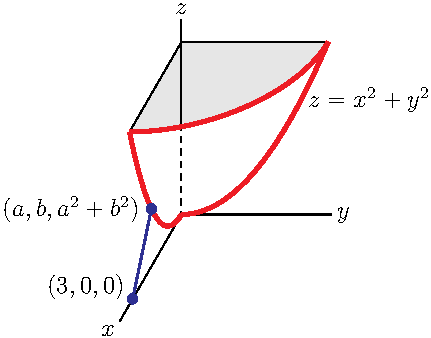
\includegraphics{distance.pdf}
\end{center}
}%
It crosses the plane at the value of $t$ which obeys
\begin{equation*}
\vn\cdot\vx(t)= c
\hskip .25 in\text{or}\hskip .25 in
\vn\cdot[\vp+t\vn]= c
\end{equation*}
namely
\begin{equation*}
t=[c-\vn\cdot\vp]/|\vn|^2
\end{equation*}
The vector
\begin{equation*}
\vx(t)-\vp=t\,\vn=\vn\,[c-\vn\cdot\vp]/|\vn|^2
\end{equation*}
has head on the plane $\vn\cdot\vx= c$, tail at $\vp$, and
is perpendicular to the plane. So the distance is the length of that
vector, which is
\begin{equation*}
|c-\vn\cdot\vp|/|\vn|
\end{equation*}
\end{solution}

%%%%%%%%%%%%%%%%%%%%%%%%%%%%%%%%%%%%
\begin{question}
Describe the set of points equidistant from $(1,2,3)$ and
$(5,2,7)$.
\end{question}

%\begin{hint}
%\end{hint}

\begin{answer}
It is the plane $x+z=8$, which is 
the plane through $(3,2,5)=\half(1,2,3)+\half(5,2,7)$ with normal 
$\llt 1,0,1\rgt=\frac{1}{4}\big(\llt 5,2,7\rgt-\llt 1,2,3\rgt \big)$.
\end{answer}

\begin{solution}
The distance from the point $(x,y,z)$ to $(1,2,3)$
is $\sqrt{(x-1)^2+(y-2)^2+(z-3)^2}$ and 
the distance from $(x,y,z)$to $(5,2,7)$ is
$\sqrt{(x-5)^2+(y-2)^2+(z-7)^2}$. Hence $(x,y,z)$ is equidistant 
from $(1,2,3)$ and $(5,2,7)$ if and only if
\begin{align*}
& & (x-1)^2+(y-2)^2+(z-3)^2&=(x-5)^2+(y-2)^2+(z-7)^2\\
&\iff & x^2-2x+1+z^2-6z+9&=x^2-10x+25+z^2-14z+49\\
&\iff & 8x+8z&=64\\
&\iff & x+z&=8
\end{align*}
This is the plane through $(3,2,5)=\half(1,2,3)+\half(5,2,7)$
with normal vector
$\llt 1,0,1\rgt=\frac{1}{4}\big(\llt 5,2,7\rgt-\llt 1,2,3\rgt \big)$.
\end{solution}

%%%%%%%%%%%%%%%%%%%%%%%%%%%%%%%%%%%%
\begin{question}
 Describe the set of points equidistant from $\va$ and $\vb$.
\end{question}

%\begin{hint}
%\end{hint}

\begin{answer}
It is the plane $2(\vb-\va)\cdot\vx=|\vb|^2-|\va|^2$,
which is the plane through $\half\va+\half\vb$
with normal vector  $\vb-\va$.
\end{answer}

\begin{solution}
The distance from the point $\vx$ to $\va$ is 
$\sqrt{(\vx-\va)\cdot(\vx-\va)}$ and the distance from $\vx$ to $\vb$ is
$\sqrt{(\vx-\vb)\cdot(\vx-\vb)}$. Hence $\vx$ is equidistant 
from $\va$ and $\vb$ if and only if
\begin{alignat*}{3}
& & (\vx-\va)\cdot(\vx-\va)&=(\vx-\vb)\cdot(\vx-\vb) \\
&\iff\qquad & |\vx|^2-2\va\cdot\vx+|\va|^2&=|\vx|^2-2\vb\cdot\vx+|\vb|^2 \\
&\iff & 2(\vb-\va)\cdot\vx&=|\vb|^2-|\va|^2
\end{alignat*}
This is the plane through $\half\va+\half\vb$
with normal vector  $\vb-\va$.
\end{solution}

%%%%%%%%%%%%%%%%%%%%%%%%%%%%%%%%%%%%
\begin{question} [M200 2003D] %1
Consider a point $P(5,-10,2)$ and the triangle with vertices
$A(0,1,1)$, $B(1,0,1)$ and $C(1,3,0)$.
\begin{enumerate}[(a)]
\item 
Compute the area of the triangle $ABC$.
\item
Find the distance from the point $P$ to the plane containing
the triangle. 
\end{enumerate}
\end{question}

%\begin{hint}
%\end{hint}

\begin{answer}
(a) $\half\sqrt{11}\approx 1.658$\qquad
(b) $\frac{3}{\sqrt{11}}\approx 0.9045$
\end{answer}

\begin{solution}
(a) One side of the triangle is 
      $\overrightarrow{AB}=\llt 1,0,1\rgt - \llt 0,1,1\rgt = \llt 1,-1,0\rgt$.
A second side of the triangle is 
      $\overrightarrow{AC}=\llt 1,3,0\rgt - \llt 0,1,1\rgt = \llt 1,2,-1\rgt$.
If the angle between $\overrightarrow{AB}$ and $\overrightarrow{AC}$
is $\theta$ and if we take $\overrightarrow{AB}$ as the base of the triangle,
then the triangle has base length $b=|\overrightarrow{AB}|$
and height $h=|\overrightarrow{AC}|\sin\theta$ and hence
\begin{equation*}
\text{area}=\half bh
=\half |\overrightarrow{AB}|\,|\overrightarrow{AC}|\sin\theta
=\half|\overrightarrow{AB}\times\overrightarrow{AC}|
=\half|\llt 1,-1,0\rgt \times \llt 1,2,-1\rgt|
\end{equation*}
As
\begin{equation*}
\llt 1,-1,0\rgt\times\llt 1,2,-1\rgt
=\det\left[\begin{matrix}
           \hi & \hj & \hk \\
            1  &  -1  &  0 \\
            1  &  2   &  -1
  \end{matrix}\right]
=\hi+\hj+3\hk
\end{equation*}
we have 
\begin{equation*}
\text{area}=\half|\llt 1,1,3\rgt|=\half\sqrt{11}\approx 1.658
\end{equation*}

(b) A unit vector perpendicular to the plane containing the 
triangle is
\begin{equation*}
\hn=\frac{\overrightarrow{AB}\times\overrightarrow{AC}}
            {|\overrightarrow{AB}\times\overrightarrow{AC}|}
=\frac{\llt 1,1,3\rgt}{\sqrt{11}}
\end{equation*}
The distance from $P$ to the plane containing the triangle is
the length of the projection of 
$\overrightarrow{AP}=\llt 5,-10,2\rgt-\llt 0,1,1\rgt
               =\llt 5,-11,1\rgt$ 
on $\hn$. If $\theta$ the angle between $\overrightarrow{AP}$
and $\hn$, then this is
\begin{equation*}
\text{distance}= |\overrightarrow{AP}|\,|\cos\theta| 
=\big|\overrightarrow{AP}\cdot\hn\big|
=\left|\llt 5,-11,1\rgt\cdot\frac{\llt 1,1,3\rgt}{\sqrt{11}}\right|
=\frac{3}{\sqrt{11}}\approx 0.9045
\end{equation*}
\end{solution}


%%%%%%%%%%%%%%%%%%%%%%%%%%%%%%%%%%%%%%%%%
\begin{question} [M200 2003A] % Bonus
Consider the sphere given by
$$
(x-1)^2+(y-2)^2+(z+1)^2=2
$$
Suppose that you are at the point $(2,2,0)$ on $S$, and you plan to follow
the shortest path on $S$ to $(2,1,-1)$. Express your initial direction
as a cross product.
\end{question}

%\begin{hint}
%
%\end{hint}

\begin{answer}
Any positive constant times
$\llt 1,1,-1\rgt\times\llt 1,0,1\rgt
=\llt 1, -2, -1\rgt$
\end{answer}

\begin{solution}
Switch to a new coordinate system with
$$
X=x-1\qquad Y=y-2\qquad Z=z+1
$$
In this new coordinate system, the sphere has equation $X^2+Y^2+Z^2=2$.
So the sphere is centred at $(X,Y,Z)=(0,0,0)$ and has radius $\sqrt{2}$.
In the new coordinate system, the initial point $(x,y,z)=(2,2,0)$
has $(X,Y,Z)=(1,0,1)$ and our final point  $(x,y,z)=(2,1,-1)$
has $(X,Y,Z)=(1,-1,0)$. Call the initial point $P$ and the final point
$Q$. The shortest path will follow the great circle from $P$ to $Q$.
\vadjust{
\begin{center}
     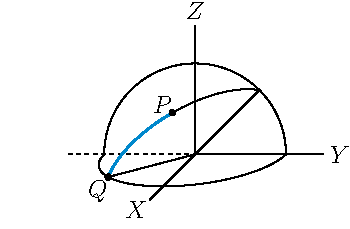
\includegraphics{OE03AQB.pdf}
\end{center}
}%
A great circle on a sphere is the intersection of the sphere with a plane
that contains the centre of the sphere. Our strategy for finding the initial
direction will be based on two observations.
\begin{itemize}
\item The shortest path lies on the plane $\Pi$ that contains the origin and the points $P$ and $Q$. Since the shortest path lies on $\Pi$,
our direction vector must also lie on $\Pi$ and hence must
be perpendicular to the normal vector to $\Pi$.
\item
The shortest path also remains on the sphere, so our initial direction
must also be perpendicular to the normal vector to 
the sphere at our initial point $P$. 
\end{itemize}
As our initial direction is perpendicular to the two normal vectors,
it is parallel to their cross product.

So our main job is to find normal vectors to the plane $\Pi$ and to the
sphere at $P$. 
\begin{itemize} 
\item One way to find a normal vector to $\Pi$ is to guess an equation for
$\Pi$. As $(0,0,0)$ is on $\Pi$, $(0,0,0)$ must obey $\Pi$'s equation.
So $\Pi$'s equation must be of the form $aX+bY+cZ=0$. That $(X,Y,Z)=(1,0,1)$ 
is on $\Pi$ forces $a+c=0$.   That $(X,Y,Z)=(1,-1,0)$ is on $\Pi$ forces 
$a-b=0$. So we may take $a=1$, $b=1$ and $c=-1$. That is, $\Pi$ is   
$X+Y-Z=0$.  (Check that all three points $(0,0,0)$, $(1,0,1)$ and
$(1,-1,0)$ do indeed obey $X+Y-Z=0$.) A normal vector to $\Pi$ is
$\llt 1,1,-1\rgt$.
\item A second way to find a normal vector to $\Pi$ is to observe that
both
\begin{itemize}
\item
the vector from $(0,0,0)$ to $(1,0,1)$, that is $\llt 1,0,1\rgt$, 
lies completely inside $\Pi$ and
\item
the vector from $(0,0,0)$ to $(1,-1,0)$, that is $\llt 1,-1,0\rgt$, 
lies completely inside $\Pi$.
\end{itemize}
So the vector
\begin{equation*}
\llt 1,0,1\rgt\times\llt 1,-1,0\rgt
=\det\left[\begin{matrix}
                     \hi & \hj & \hk \\
                     1   &  0  & 1 \\
                     1   &  -1  & 0
                \end{matrix}\right]
=\hi + \hj -\hk
\end{equation*}
is perpendicular to $\Pi$.
\item
The vector from the centre of the sphere to the point $P$ on the sphere
is perpendicular to the sphere at $P$. So a normal vector to 
the sphere at our initial point $(X,Y,Z)=(1,0,1)$ is $\llt 1,0,1\rgt$.
\end{itemize}
Since our initial direction\footnote{Note that the change of coordinates
$X=x-1$, $Y=y-2$, $Z=z+1$ has absolutely no effect on any velocity or direction
vector. If our position at time $t$ is $(x(t),y(t),z(t))$ in the
original coordinate system, then it is $(X(t),Y(t),Z(t))
=(x(t)-1,y(t)-2,z(t)+1)$ in the new coordinate system. The velocity
vectors in the two coordinate systems $\llt x'(t),y'(t),z'(t)\rgt
=\llt X'(t),Y'(t),Z'(t)\rgt$ are identical.}
must be perpendicular to both $\llt 1,1,-1\rgt$ and $\llt 1,0,1\rgt$, 
it must be one of  $\pm\llt 1,1,-1\rgt\times\llt 1,0,1\rgt$. 
To get from $(1,0,1)$ to $(1,-1,0)$ by the shortest path, our $Z$ 
coordinate should decrease from $1$ to $0$. So the $Z$ coordinate of 
our initial direction should be negative. This is the case for 
\begin{equation*}
\llt 1,1,-1\rgt\times\llt 1,0,1\rgt
=\det\left[\begin{matrix}
                     \hi & \hj & \hk \\
                     1   &  1  & -1 \\
                     1   &  0  &  1
                \end{matrix}\right]
=\hi - 2\,\hj -\hk
\end{equation*}
\end{solution}

